\begin{adjustwidth*}{}{-2.25in}
\textbf{{\large Exercises}}
\setlength{\columnsep}{25pt}
\begin{multicols*}{2}
\noindent Terms and Concepts \small
\begin{enumerate}[1)]
\item T/F: An ``optimization problem'' is essentially an ``extreme values'' problem in a ``story problem'' setting.
\item T/F: This section teaches one to find the extreme values of function that have more than one variable.
\end{enumerate} 

\noindent {\normalsize Problems} \small

\begin{enumerate}[1),resume]
\item Find the maximum product of two numbers (not necessarily integers) that have a sum of $100$.
\item Find the minimum sum of two numbers whose product is $500$.
\item Find the maximum sum of two numbers whose product is $500$.
\item Find the maximum sum of two numbers, each of which is in $[0,300]$ whose product is $500$.
\item Find the maximal area of a right triangle with hypotenuse of length $1$. 
\item A rancher has $1000$ feet of fencing in which to construct adjacent, equally sized rectangular pens. What dimensions should these pens have to maximize the enclosed area?

\noindent\begin{minipage}{\linewidth}
\centering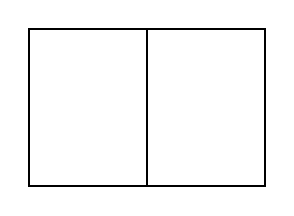
\begin{tikzpicture}
\draw [thick](0,0) rectangle (3,2);
\draw [thick](1.5,0) -- (1.5,2);
\end{tikzpicture}
\end{minipage}

\item A standard soda can is roughly cylindrical and holds $355$ cm$^3$ of liquid. What dimensions should the cylinder be to minimize the material needed to produce the can? Based on your dimensions, determine whether or not the standard can is produced to minimize the material costs.
\item Find the dimensions of a cylindrical can with a volume of $206$ in$^3$ that minimizes the surface area.

The ``\#10 can''is a standard sized can used by the restaurant industry that holds about $206$ in$^3$ with a diameter of $6 \frac{2}{16}$ in and height of $7$ in. Does it seem these dimensions where chosen with minimization in mind?

\item The strength $S$ of a wooden beam is directly proportional to its cross sectional  width $w$ and the square of its height $h$; that is, $S = kwh^2$ for some constant $k$. 

\noindent\begin{minipage}{\linewidth}
\centering
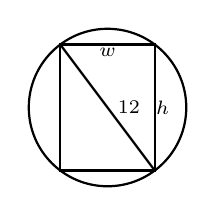
\begin{tikzpicture}
\draw [thick](0,0) circle (1cm);
\draw [thick](-.6,.8) -- node [pos=.5,right] {\scriptsize $12$} (.6,-.8);
\draw [thick](-.6,-.8) rectangle (.6,.8);
\draw (.7,0) node {\scriptsize $h$} (0,.7) node {\scriptsize $w$};
\end{tikzpicture}
\end{minipage}

Given a circular log with diameter of $12$ inches, what sized beam can be cut from the log with maximum strength?

\item A power line is to be run to an offshore facility in the manner described in Example~\ref{Ex:3.4.Eg3}. The offshore facility is $2$ miles at sea and $5$ miles along the shoreline from the power plant. It costs \$ $50,000$ per mile to lay a power line underground and \$ $80,000$ to run the line underwater. 

How much of the power line should be run underground to minimize the overall costs?
\item A power line is to be run to an offshore facility in the manner described in Example~\ref{Ex:3.4.Eg3}. The offshore facility is $5$ miles at sea and $2$ miles along the shoreline from the power plant. It costs $\$50,000$ per mile to lay a power line underground and $\$80,000$ to run the line underwater. 

How much of the power line should be run underground to minimize the overall costs?

\item A woman throws a stick into a lake for her dog to fetch; the stick is $20$ feet down the shore line and $15$ feet into the water from there. The dog may jump directly into the water and swim, or run along the shore line to get closer to the stick before swimming. The dog runs about $22$ ft/s and swims about $1.5$ ft/s. 

How far along the shore should the dog run to minimize the time it takes to get to the stick?

\item A woman throws a stick into a lake for her dog to fetch; the stick is $15$ feet down the shore line and $30$ feet into the water from there. The dog may jump directly into the water and swim, or run along the shore line to get closer to the stick before swimming. The dog runs about $22$ ft/s and swims about $1.5$ ft/s. 

How far along the shore should the dog run to minimize the time it takes to get to the stick? \textit{(Google ``calculus dog'' to learn more about a dog's ability to minimize times.)}

\item What are the dimensions of the rectangle with largest area that can be drawn inside the unit circle?

	\item A rectangular box with a square bottom and closed top is to be made from two materials.  The material for the side costs $\$1.50$ per square foot and the material for the bottom costs $\$3.00$ per square foot.  If you are willing to spend $\$15$ on the box, what is the largest volume it can contain?  Justify your answer completely using calculus.

\end{enumerate}

%------------------------------------------
% END OF EXERCISES ON FIRST PAGE
%------------------------------------------
\end{multicols*}
\end{adjustwidth*}

\clearpage

\begin{adjustwidth*}{}{-2.25in}
\setlength{\columnsep}{25pt}
\begin{multicols*}{2}\small

\begin{enumerate}[1),start=18]
	\item A farmer wants to start raising cows, horses, goats, and sheep, and desires to have a rectangular pasture for the animals to graze in.  However, no two different kinds of animals can graze together.  In order to minimize the amount of fencing she will need, she has decided to enclose a large rectangular area and then divide it into four equally sized pens, or grazing areas.  She has decided to purchase $7500$ ft of fencing.  What is the maximum possible area that each of the four pens will enclose?
	\item Two vertical towers of heights $60$ ft and $80$ ft stand on level ground, with their bases $100$ ft apart.  A cable that is stretched from the top of one pole to some point on the ground between the poles, and then to the top of the other pole.   What is the minimum possible length of cable required?  Justify your answer completely using calculus.
	\item A company is designing propane tanks that are cylindrical with hemispherical ends.   Assume that the company wants tanks that will hold $1000$ cubic feet of gas, and that the ends are more expensive to make, costing $\$5$ per square foot, while the cylindrical barrel between the ends costs $\$2$ per square foot.  Use calculus to determine the minimum cost to construct such a tank.
\end{enumerate}

%---------------------------------------------
% END OF EXERCISES ON SECOND PAGE
%---------------------------------------------
\end{multicols*}
\end{adjustwidth*}

\afterexercises